\section{Persistent Homology by probability}

While persistence by height allows us to do some basic accounting and comparisons, it is not capturing the graph connectivity questions we are after.  
Nor does it allow us to explore the taint tree probabilistically.
All transactions at a given time occupy the same set, they are not distinguishable one from the other.
We introduce another construction that lets us try to connect with graph approaches to the analysis.

We will need a notion for distance, and we refer to the cdfs and fits computed in the fit section to do so.
In the Ring object instantiation we require a set of decoys \textit{and} a reference tx, we label txo for origin transaction.  
This allows us to do a few things.  
The ring needn't be required to actually exist somewhere on the blockchain, we can instantiate it with a different txo and place the ring in the context of a different txo.
It is the case that rings have been re-used for different transactions \footnote{Isthmus, Rucknium private communications}, but they will still differ by different txo (must also differ in the real input too), and different hash.

These different txos change the offset, how long one must integrate to get the proper cdf, and thus the probabilities will be shifted monotonically as well.  
Furthermore, we can take as input a height persistogram, along with some parameter, to find a different tx that could be `confused' with our tx (as in occupy the same simplex, and thus point to the same representative).
This parameter when set to zero will force the sampled tx to have come from the same block as the target tx, and the probabilities will be identical.

The evaluations of the cdf in particular we are interested in are the integral of the pdf from time zero (the height of the txo) to the time of the height of the ring constituent.  
These give us the probabilities of the constituents being the real transaction.
We can also consider the relative probabilities by normalizing; dividing by the sum of the evaluated cdfs.
This has the more intuitive intrpretation of a weighted (currently) 16 sided dice.  

We pivot to a distance notion by taking $1-q$ rather than q, so more likely things are the ones closer together, and certaicornties resolve on top of each other.

The registry objects, basically just a dictionary with keys the tx hash and values the tx object, can be used to construct the distance matrices we need to compute the homologies, or other graph metrics.
We can recover spectra and other metrics for the corresponding graphs (1-skeletons) by setting the distance to one for each ring constituent.

A first attempt at constructing these matrices is included in the Taint-Explorer notebook.
    


\subsection{Taint Trees}

Persistence works a little bit differently than your intuition might have for probabilities.  
For example a path two-hops deep with .9 connecting the first and .9 connecting the second has probability of .81 of occurring, yet the two txs will already be connected when the filtration parameter reaches .9.  

\subsection{Sampling Paths}

To sample paths each ring has a pymc categorical distribution over the RingCT that we can draw from.  This distribution is also called in calls to the value of a ring or tx.
We have considered all paths with equal opportunity at this stage.  
Fig. \ref{fig:ptoc} shows a histogram of 3300 paths to coinbase from a transaction.  
We haven't parameterized this histogram at this stage, but we expect it to be exponential with mean related to the probability of drawing a coinbase transaction out of the ring, which terminates the sampling path.
We can construct persistence diagrams for any of these paths, height paths are used to show the four diagrams in Table \ref{tab:pdsSP}.
For a given decoy selection algorithm, (or series, since this changes with block height), we can evaluate the likelihood of a given path to occur.  
Dynamic partition functions, that are weighted path integrals like this here, are called Maximum Caliber and have utility in statistical mechanics when the observables observed are not the energy paramater, but a categorical state (folded/unfolded, orbiting stationary points A,B,C etc. ). 
These diagrams are used to estimate the value of a given tx, and to probabilistically sample the taint tree.
  
We can also look at a distribution of the values of the coinbases at \ref{fig:valsc}.
We expect taint trees of different txes with common true source to have comparable statistics.  
We need to check if transactions which could have been used interchangably as a decoy, also generate similar statistics.
As mentioned in the Value section, these distrubitons of coinbases can be used to generate a probabilistic notion of value of an unknown tx.

\begin{figure}[h]
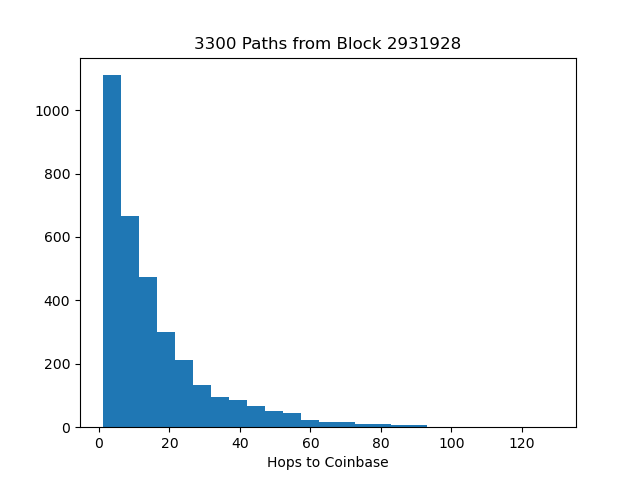
\includegraphics[scale=0.5]{pathstocoinbase}
\caption{A histogram of the length it takes to get to a coinbase, drawn from 3300 samples of a single transaction.  These values can be used in the value expectation}
\label{fig:ptoc}
\end{figure}

\begin{center}
\begin{table}
\begin{tabular}{|c|c|}

\hline
 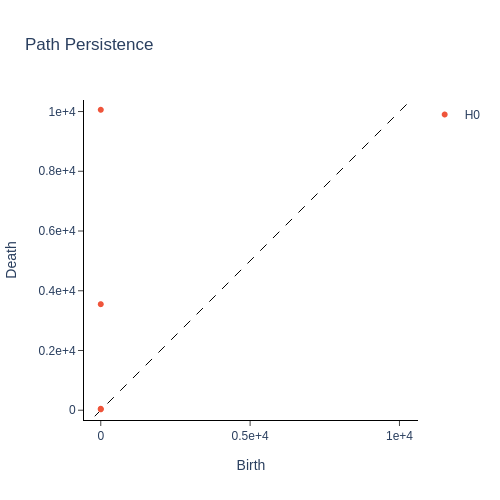
\includegraphics[scale=0.3]{pds_0} & 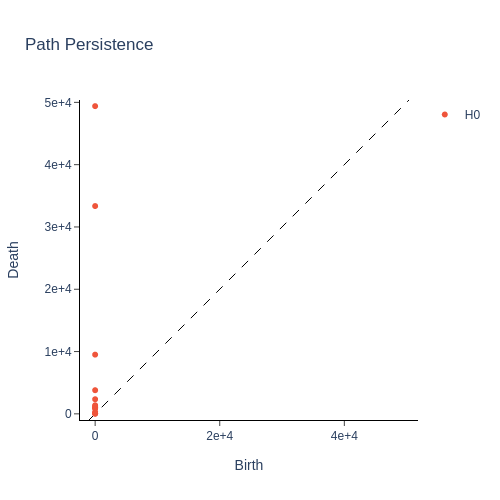
\includegraphics[scale=0.3]{pds_1}  \\ \hline
  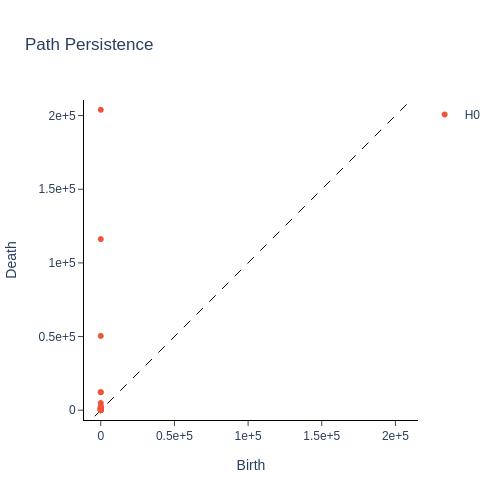
\includegraphics[scale=0.3]{pds_2} & 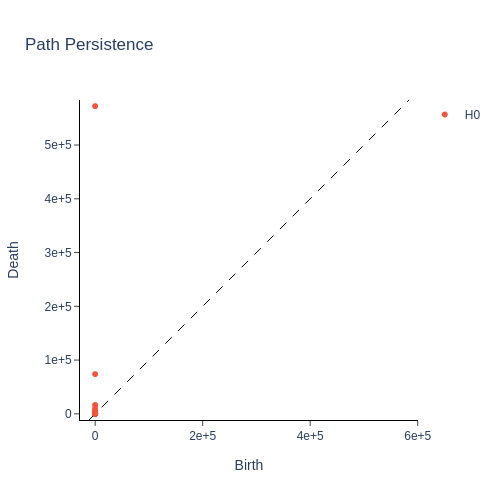
\includegraphics[scale=0.3]{pds_3}  \\ \hline
\end{tabular}
\caption{Persistence diagrams of four sampled paths to coinbase.  Diagrams with a few points have short trips to coinbase, diagrams with a lot of points have a lot of transactions prior to making it to coinbase.  The spacings within the diagram specifies how large of block jumps were required to make it there.}
\label{tab:pdsSP}
\end{table}
\end{center}

\begin{figure}[h]
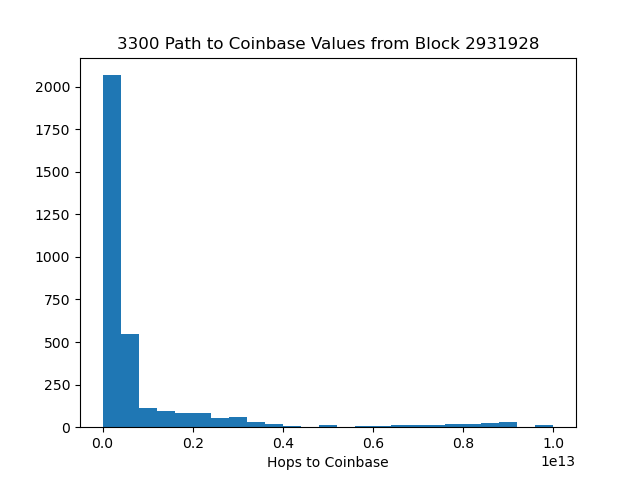
\includegraphics[scale=0.5]{valscoinbase}
\caption{A distribution of the values at coinbase of the separate paths.  
An estimate of the value of an unknown tx is the mean of this distribution times the number of inputs divided by the number of outputs.}
\label{fig:valsc}
\end{figure}
